% Tipo de documento
\documentclass[12pt,twocolumn,a4paper]{report}
% UTF-8 and friends
\usepackage[utf8]{inputenc}
\usepackage[spanish]{babel}
\usepackage{titlesec}
\usepackage{titletoc}
\usepackage{hyperref}
\usepackage{lipsum}
\usepackage{multicol}
\usepackage{graphicx}
\usepackage{float}
\usepackage{amsmath}
\usepackage{vmargin}
\usepackage{tcolorbox}
\tcbuselibrary{theorems}
\usepackage[colorinlistoftodos,textwidth=2cm,shadow]{todonotes}
\usepackage{cancel}
\setpapersize{A4}
\setmargins{2.5cm}       % margen izquierdo
{1.5cm}                        % margen superior
{16.5cm}                      % anchura del texto
{23.42cm}                    % altura del texto
{10pt}                           % altura de los encabezados
{1cm}                           % espacio entre el texto y los encabezados
{0pt}                             % altura del pie de página
{2cm}                           % espacio entre el texto y el pie de página
% Para los capitulos
%\titleformat{\chapter}[display]
%{\bfseries\huge\bfseries\filcenter}{\thechapter}{25pt}{\Large}
% [%
%  \startcontents
%  \printcontents{}{1}{\setcounter{tocdepth}{3}}%
%  ]
\title{Apuntes de Termodinámica}
\date{}

\begin{document}
\maketitle

\newpage
\tableofcontents

%----------------------------------------------------
\onecolumn
\chapter*{Introducción}
\addcontentsline{toc}{chapter}{Introducción}
El presente apunte es el comienzo de un proyecto personal, el cual tiene como objetivo llevar donde quiera que vaya los apuntes de las clases de todos mis ramos universitarios. 

Comenzaré con termodinámica, ¿Qué es la termodinámica?, pues es la ciencia completamente empírica que describe mascroscópicamente las propiedades de los sistemas en equilibrio. 

\twocolumn
\newpage


\chapter*{Conceptos Fundamentales}
\addcontentsline{toc}{chapter}{Conceptos Fundamentales}
	\section*{Sistema}
\addcontentsline{toc}{section}{Sistema}
Cantidad de materia o una región en el espacio elegida para estudio. La masa o región fuera del sistema recibe el nombre de alrededores o medio ambiente. (Entorno o medio)
\begin{figure}[H]
\centering
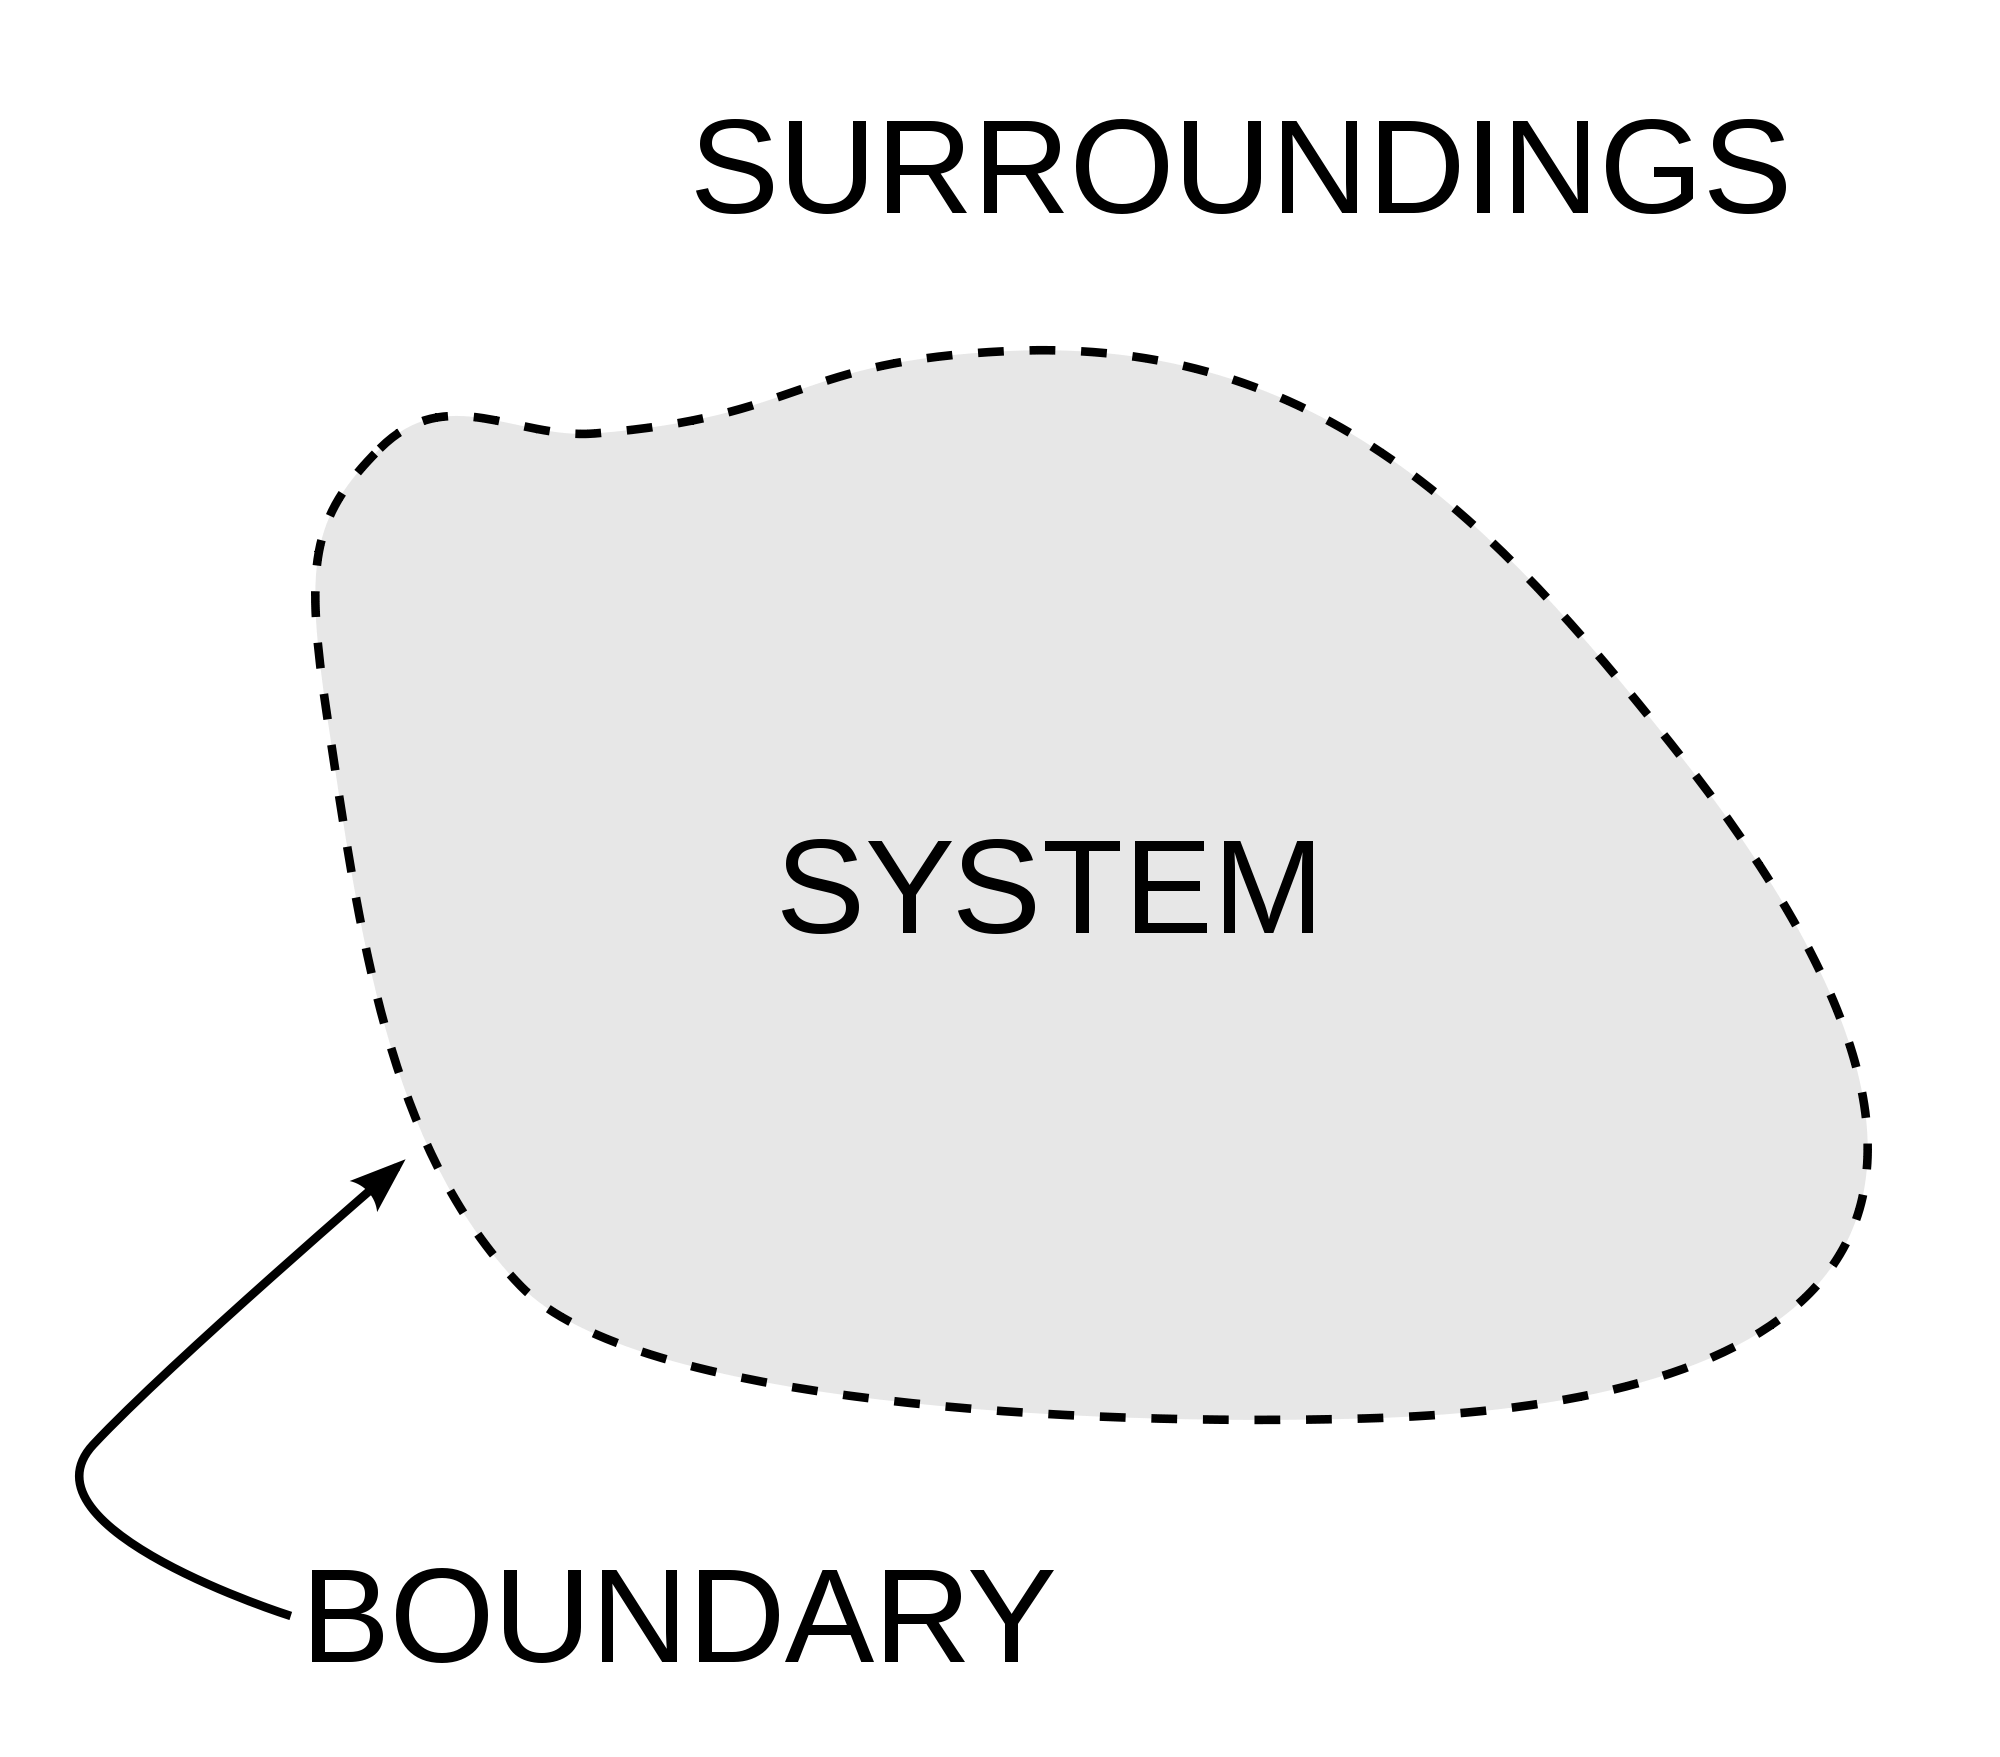
\includegraphics[scale=0.05]{graficos/sistema1.jpeg}
\end{figure}


	\section*{Límite del sistema}
\addcontentsline{toc}{section}{Límite del sistema}
Superficie o pared o frontera que delimita al sistema, la cual puede ser física o imaginaria, variable o invariable en su forma y/o volumen, adiabática o diatérmico.

	\section*{Universo}
\addcontentsline{toc}{section}{Universo}
Se define simplemente como el sistema unido al  ambiente.

	\section*{Tipos de Sistemas}
	\addcontentsline{toc}{section}{Tipos de Sistemas}
Los sistemas por sus interacciones con el medio, se clasifican en cerrados, abiertos y aislados: 
	\begin{itemize}
	\item{\textbf{Abierto:}	Aquel que puede intercambiar materia y energia.
	\begin{figure}[H]
	\centering	
	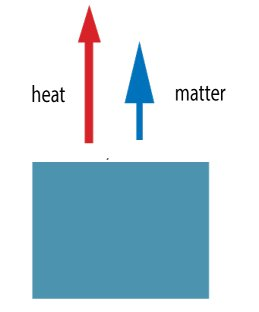
\includegraphics[scale=0.3]{graficos/tiposdesistemas1.jpeg}	
\end{figure}}	
	\item{\textbf{Cerrado:} Aquel sistema que no puede intercambiar materia con el medio, pero sí energía.
	\begin{figure}[H]
	\centering	
	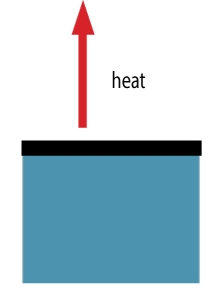
\includegraphics[scale=0.32]{graficos/tiposdesistemas2.jpeg}	
\end{figure}}	
	\item{\textbf{Aislado:} No se produce intercambio alguno de materia ni energia con el medio.
	\begin{figure}[H]
	\centering	
	
\includegraphics[scale=0.3]{graficos/tiposdesistemas3.jpeg}	
\end{figure}}	
	\end{itemize}
	\section*{Fluido}
	\addcontentsline{toc}{section}{Fluido}
	No resiste a la deformación, ofrece pequeña/nula resistencia a las fuerzas constantes. 
	\section*{Densidad($\rho$)}
	\addcontentsline{toc}{section}{Densidad($\rho$)}
	Cantidad de masa contenida en un volumen. Matemáticamente se define como
	\begin{equation*}
	\rho = \frac{m}{V}
	\end{equation*}
	\section*{Presión}
	\addcontentsline{toc}{section}{Presión}
	Fuerza(magnitud) por unidad de área, que actúa perpendicularmente a una superficie. Matemáticamente se expresa como
	\begin{equation*}
	P = \frac{F}{A}
	\end{equation*}
	
	
		 
\onecolumn

\chapter*{Estados de un sistema}
\addcontentsline{toc}{chapter}{Estados de un sistema}
\section*{Coordenadas termodinámicas}
\addcontentsline{toc}{section}{Coordenadas Termodinámicas}
Son aquellas coordenadas macroscópicas que son independientes de cualquier marco de referencia y que sólo describen los aspectos internos del sistema.
\section*{Sistema Termodinámico}
\addcontentsline{toc}{section}{Sistema Termodinámico}
Aquel sistema que puede ser descrito en términos de sus coordenadas termodinámicas.
\section*{Estado de un sistema}
\addcontentsline{toc}{section}{Estado de un sistema}
Queda determinado por los valores de ciertas magnitudes medibles experimentalmente denominadas coordenadas termodinámicas o propiedades o variables de estado. Ej: Presión, volumen, Temperatura, etc.
\section*{Pared Adiabática}
\addcontentsline{toc}{section}{Pared Adiabática}
Capa ideal que impide toda variación de temperatura del sistema. Esta tapa no permite el intercambio de material ni el flujo de calor. Ej: Capas de hormigón, lona de vidrio.
\section*{Pared Diatérmica}
\addcontentsline{toc}{section}{Pared Diatérmica}
Permiten el flujo de calor pero no el intercambio de materia. Ej: lámina delgada de cobre.




\twocolumn


\chapter*{Equilibrio térmico, temperatura y procesos}
\addcontentsline{toc}{chapter}{Equilibrio térmico y temperatura}
El concepto de temperatura tiene su origen en las percepciones sensoriales del hombre. Puede vincularse con la sensación relativa de calor y frio.

Para alcanzar una medición objetiva del sentido de la temperatura, hay que establecer un criterio de igualdad de temperatura.

Consideremos el siguiente ejemplo: Dos bloques A y B del mismo material. Nuestro tacto nos dice que A está más caliente que B. Si A y B se ponen en contacto uno con el otro, encontramos que después de un tiempo suficiente, los dos parecen estar a igual temperatura. Entonces,
\todo[inline,backgroundcolor=red!10]{Se dice que A y B se encuentran en equilibrio térmico (tienen la misma temperatura)} 
\section*{Equilibrio térmico}
\addcontentsline{toc}{section}{Equilibrio térmico}
Estado en el cual la temperatura del sistema es la misma en todos los puntos. \textbf{Igualdad de T en todos los puntos}

Todos los objetos ordinarios poseen una propiedad física que determina si están o no en equilibrio térmico con otros objetos en contacto. Esta propiedad es la temperatura.

Supongamos que tenemos un sistema arbitrario \textbf{aislado} y abandonado a sí mismo: 
\begin{itemize}
  \setlength\itemsep{0.001cm}
  \item {Si es que existen diferencias de temperatura, logrará el equilibrio térmico}
  \item {Si es que existen, inicialmente, diferencias de presión, logrará el equilibrio mecánico}
  \item {Luego de un tiempo, existirá el equilibrio químico y las reacciones van a cesar}
\end{itemize}

\subsection*{Ley cero de la Termodinámica}
\addcontentsline{toc}{subsection}{Ley cero de la Termodinámica}
Si dos cuerpos, A y B, por separado están en equilibrio térmico con un tercer cuerpo C, entonces A y B están en equilibrio térmico entre sí. 

\todo[inline,backgroundcolor = green!10]{Los cuerpos A y B están en equilibrio térmico si poseen igual temperatura}

\section*{Temperatura}
\addcontentsline{toc}{section}{Temperatura}
Está directamente relacionada \textbf{con la energía cinética de los átomos y moléculas que componen dicho objeto}. Nuestra compresión de lo frío o caliente es sólo una \textbf{medida de la rapidez con la que intercambian energía los objetos}

\section*{Procesos}
\addcontentsline{toc}{section}{Procesos}
Cuando alguna de las propiedades del sistema cambia, el estado del sistema se modifica y se dice que experimenta un proceso de transformación

\subsection*{Proceso cuasiestático}
\addcontentsline{toc}{subsection}{Proceso cuasiestático}
Si el proceso se realiza de modo que en cada instante el sistema difiere \textbf{sólo infenitesimalmente} de un estado de equilibrio. Se aproxima sólo a una sucesión de estados de equilibrio.

\subsection*{Proceso no cuasiestático}
\addcontentsline{toc}{subsection}{Proceso no cuasiestático}
Si existen diferencias finitas con el equilibrio. Todos los procesos reales son no cuasiestáticos.

\subsection*{Proceso isocórico}
\addcontentsline{toc}{subsection}{Proceso isocórico}
Cuando el \textbf{volumen} permanece constante

\subsection*{Proceso isobárico}
\addcontentsline{toc}{subsection}{Proceso isobárico}
Cuando la \textbf{presión} permanece constante


\subsection*{Proceso isotérmico}
\addcontentsline{toc}{subsection}{Proceso isotérmico}
Cuando la \textbf{temperatura} permanece constante

\begin{figure}[H]
	\centering	
	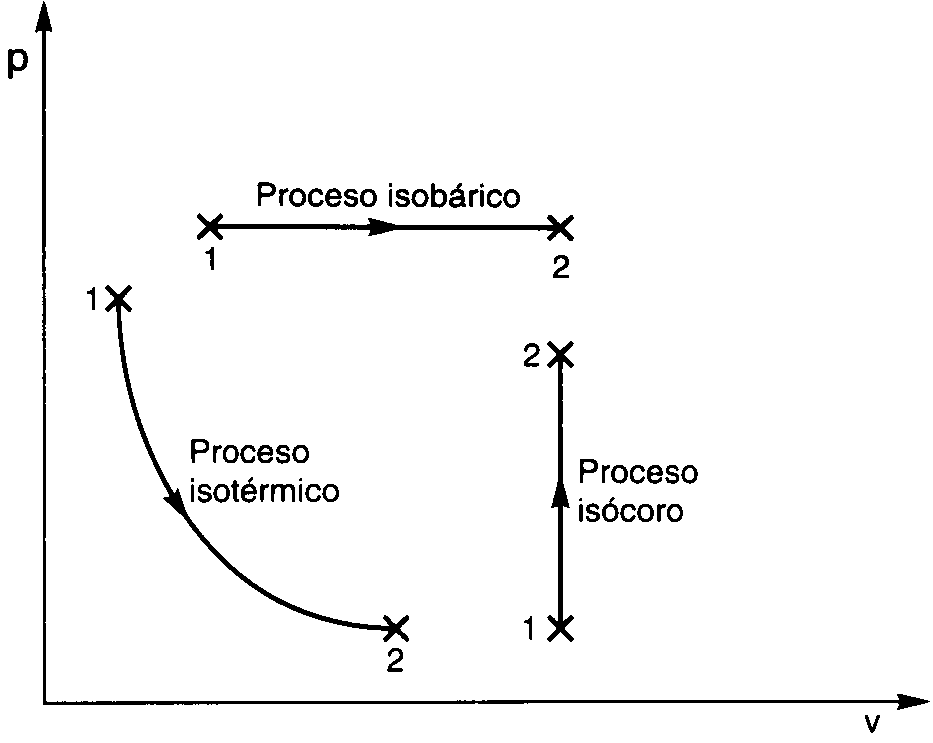
\includegraphics[scale=0.25]{graficos/todos.jpeg}	
\end{figure}

\section*{Variación de la presión con la profundidad}
\addcontentsline{toc}{section}{Variación de la presión con la profundidad}
Un fluido se encuentra en reposo en un recipiente cuando
Todas las partes del fluído estan en equilibrio hidrostático y todos los puntos que están a la misma profundidad tienen la misma presión.

Supongamos que un objeto en un fluido ha alcanzado el equilibrio hidrostático y queremos saber la presión hidrostática.  
\begin{figure}[H]
	\centering	
	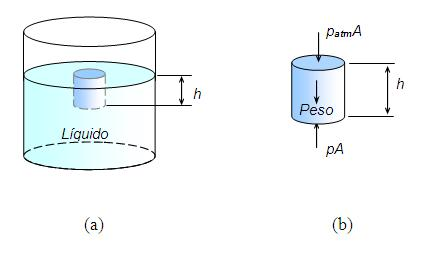
\includegraphics[scale=0.85]{graficos/hidrostatica.jpeg}	
\end{figure}

La presión atmosférica es $P_o$ y, como el objeto ha alcanzado el equilibrio, la presión ejercida por el fluido será $F = P\cdot A$. Por sumatoria de fuerzas tenemos
\begin{equation*}
\sum F_y = P_o \cdot A + mg = P\cdot A,
\end{equation*}
sin embargo, podemos expresar la masa como
\begin{align*}
m &= \rho \cdot V \\
  &= \rho \cdot Ah
\end{align*}
así,
\begin{equation*}
P\cdot A - P_o \cdot A - mg = 0
\end{equation*}


\begin{equation*}
\tcboxmath[colback=teal!50!white,colframe=black]{
P=P_o + \rho gh}
\end{equation*}








\chapter*{Ecuación de Estado (EdE)}
\addcontentsline{toc}{chapter}{Ecuación de Estado (EdE)}
El estado de una cierta masa $m$ está determinada por su presión (P), Temperatura(T) y volumen (V). En general, estas cantidades no pueden variar todas ellas independientemente. 

En términos matemáticos, existe una relación funcional entre estas cantiades que puede representarse simbólicamente como:
\begin{equation*}
f(P,V,T,m) = 0
\end{equation*}
o también como 
\begin{equation*}
f(P,v,T) = 0
\end{equation*}
en este caso $v = \dfrac{V}{m}$
\section*{EdE de un Gas Ideal}
\addcontentsline{toc}{section}{EdE de un Gas Ideal}
¿Qué es un gas ideal?. Pues básicamente es un modelo idealizado que representa muy bien el comportamiento de los gases en algunas circunstancias y peor en otras. 

En general, el comportambiento de un gas se aproxima más al modelo del gas ideal \textbf{a muy bajas presiones, cuando las moléculas están separadas entre sí.} 

\subsection*{Formulación de las leyes de los gases ideales}
\addcontentsline{toc}{subsection}{Formulación de las leyes de los gases ideales}
\begin{itemize}
\setlength\itemsep{0.001cm}
\item{\textbf{Robert Boyle:}Observó que a temperatura constante, el volumen de una cantidad fija de gas es inversamente proporcional a su presión:
\begin{equation*}
V \alpha \thinspace \dfrac{1}{P} 
\end{equation*}
o
\begin{equation*}
PV = cte
\end{equation*}}
\item{\textbf{Joseph Gay-Lussac:}Concluye que si la presión del gas se mantiene constante, el volumen de éste no varía linealmente con la temperatura. Si los experimentos se llevan a cabo a presiones no demasiado elevadas, se obtienen rectas diferentes, una para cada presión, que se cortan en un punto común que, según puede obtenerse por extrapolación, corresponde a una temperatura de \textbf{-273.15 C}. Su ley establece que:
\begin{equation*}
\dfrac{V}{T} = cte
\end{equation*}}
\item{\textbf{Amadeo Avogadro:} Establece que \textbf{Volúmenes iguales de gases a la misma temperatura y presión contienen el mismo número de moléculas}. Con esto se concluye que:
\begin{equation*}
V \alpha \thinspace n
\end{equation*}}
\end{itemize}

Las relaciones anteriores, basadas en la observación experimental pueden combinarse gloriosamente en una sola:
\begin{equation*}
PV \alpha \thinspace nT
\end{equation*}

Como vemos, esto es una proporcionalidad, osea que hace falta una constante. Pues bien, para calcularla se efectuaron medidas del volumen de una cantidad conocida de gas a distintas temperaturas y presiones, y\textbf{extrapolando a presión cero, que es donde se cumplen exactamente las leyes de los gases ideales, se obtiene:}
\begin{equation*}
\displaystyle\lim_{p\to 0}(\dfrac{PV}{nT}) = R
\end{equation*}
Este límite es llamado \textbf{Constante universal de los gases = R}
\begin{itemize}
\setlength\itemsep{0.001cm}
\item {$R = 0.08206$ atm L/mol K}
\item {$R = 8.3143$ J/mol K}
\item {$R = 8.3143 \times 10^3$ J/kilomol K}
\end{itemize}

\subsection*{Las hermosas ecuaciones}
\addcontentsline{toc}{subsection}{Las hermosas ecuaciones}
Las ecuaciones que gobiernan en un gas ideal son 
\begin{equation*}
PV = nRT
\end{equation*}
o
\begin{equation*}
Pv = RT
\end{equation*}
donde
\begin{equation*}
v = \dfrac{V}{n}
\end{equation*}

\subsection*{Superficie PVT para un gas ideal}
\addcontentsline{toc}{subsection}{Superficie PVT para un gas ideal}
Como la EdE para una masa dada de una sustancia es una relación entre las tres variables P,V y T, define una superficie en un sistema de coordenadas rectangulares en el que P,V y T están representadas a lo largo de los tres ejes.
\begin{figure}[H]
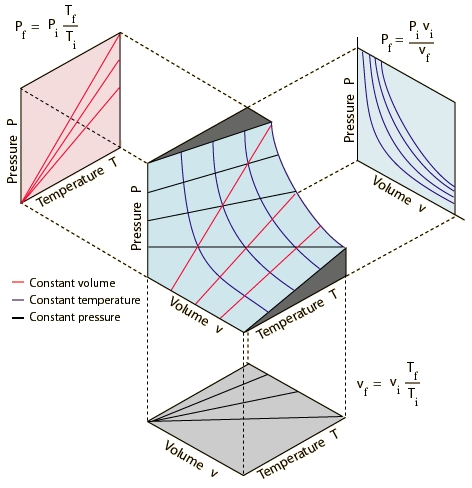
\includegraphics[scale=0.5]{graficos/pvt.jpeg}
\end{figure}

\section*{EdE de gases reales}
\addcontentsline{toc}{section}{EdE de gases reales}
Se han propuesto muchas ecuaciones que describen las relaciones P-V-T de los gases con más exactitud de un gas ideal. 
\subsection*{EdE de van der Waals}
\addcontentsline{toc}{subsection}{EdE de van der Waals}
\begin{equation*}
\left(P + \dfrac{a}{v^2}\right)(v - b) = RT
\end{equation*}
o 
\begin{equation*}
\left(P + \dfrac{an^2}{V^2}\right)(V - nb) = nRT
\end{equation*}
donde $v \equiv \dfrac{V}{n}$
En estas ecuaciones
\begin{itemize}
\setlength\itemsep{0.001cm}
\item{a y b: Son constantes empíricas. Difieren de un gas a otro}
\item{b: Representa aproximadamente \textbf{el volumen de un mol de moléculas}. El volumen total de moléculas es nb}
\item{V-nb: Volumen neto disponible para que se muevan (ya que nb representa la reducción del volumen debido al tamaño finito de las moléculas}
\item{a: Depende de las fuerzas de atracción intermoleculares}
\end{itemize}
\todo[inline,backgroundcolor=red!10]{Cuando n/V es un valor pequeño, la distancia media entre las moléculas es grande y la EdE se reduce a la del gas ideal}

\section*{Derivadas parciales, dilatación y compresibilidad}
\addcontentsline{toc}{section}{Derivadas parciales, dilatación y compresibilidad}
Podemos imaginar la EdE de forma que una coordenada aparezca en función de las otras dos. Así, 
\begin{equation*}
V = f(T,P)
\end{equation*}
Un cambio infinitesimal de un estado de equilibrio a otro implica cambios dV, dT y dP. Un teorema fundamental del cálculo de derivadas parciales permite escribir:
\begin{equation*}
dV = \left(\frac{\partial V}{\partial T}\right)_P dT + \left(\frac{\partial V}{\partial P}\right)_T dP
\end{equation*}
donde dV: es el diferencial total(la diferencia total de una función real de diversas variables reales corresponde a una combinación lineal de diferenciales cuyos coeficientes son los gradientes de la función).

\section*{Coeficiente de dilatación cúbica}
\addcontentsline{toc}{section}{Coeficiente de dilatación cúbica}
La dependencia del volumen de un sólido, líquido o gas con la temperatura a presión constante viene dada por: 
\begin{equation*}
\beta = \dfrac{1}{V}\left(\frac{\partial V}{\partial T}\right)_P [K]^{-1}
\end{equation*}
\textbf{NOTA:} El valor de $\beta$ indica cómo varia el columen cuando varía la temperatura a presión constante.
\vspace{5px}
\todo[inline,backgroundcolor=red!10]{El valor de $\beta$ es difiere en cada sustancia. Para gases y sólidos es \textbf{siempre positivo}, para líquidos es \textbf{casi siempre positivo}}
\subsection*{Coeficiente de dilatación media}
\addcontentsline{toc}{subsection}{Coeficiente de dilatación media}
Para un intervalo finito de temperaturas entre $T_1$ y $T_2$ viene dado por (a P constante): 
\begin{equation*}
\bar{\beta}=\dfrac{1}{V_1}\left(\frac{V_2 - V_1}{T_2 - T_1}\right)
\end{equation*}
\section*{Compresibilidad isoterma}
\addcontentsline{toc}{section}{Compresibilidad isoterma}
La dependencia del volumen de un sólido, líquido o gas con la presión  a temperatura constante viene dada por:  
\begin{equation*}
\kappa=-\dfrac{1}{V}\left(\frac{\partial V}{\partial P}\right)_T [Pa]^{-1}
\end{equation*}
\vspace{5px}
\todo[inline,backgroundcolor=green!10]{El signo negativo se debe a que el volumen siempre disminuye al aumentar la presión. $\left(\frac{\partial V}{\partial P}\right)_T$ es negativo. Este coeficiente resulta siempre positivo}
\subsection*{Compresibilidad media}
\addcontentsline{toc}{subsection}{Compresibilidad media}
A temperatura constante
\begin{equation*}
\kappa=-\dfrac{1}{V_1}\left(\frac{V_2 - V_1}{P_2 - P_1}\right)
\end{equation*}

\chapter*{Trabajo (W)}
\addcontentsline{toc}{chapter}{Trabajo(W)}
Cuando un sistema termodinámico experimenta un proceso, el trabajo que se realiza puede asociarse siempre a alguna fuerza. Sin embargo, es conveniente expresar el trabajo en función de las propiedades termodinámicas del sistema.

\section*{Expansión Cuasiestática}
\addcontentsline{toc}{section}{Expansión Cuasiestática}
Consideremos un sistema hidroestático contenido en un cilindro provisto de un pistón móvil sobre el cual pueden actuar el sistema y el medio.
\begin{figure}[H]
\centering
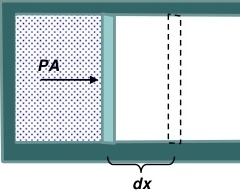
\includegraphics[scale=0.5]{graficos/trab1.jpeg}
\end{figure}
donde 
\begin{itemize}
\setlength\itemsep{0.001cm}
\item{P: Presión ejercida por el sistema sobre el pistón}
\item{PA: fuerza}
\item{dx: distancia que se mueve el pistón en la dirección de la fuerza}
\end{itemize}
El sistema realiza una cantidad infenitesimal del trabajo d'W 
\begin{align*}
d'W &= PA\thinspace dx \\
d'v &= A\thinspace dx 
\end{align*}
por lo tanto 
\begin{equation*}
d'W = P\thinspace dv 
\end{equation*}

El trabajo total realizado por el gas cuando el volumen varía desde $V_a$ a $V_b$ viene dado por
\begin{equation*}
W = \int_{V_a}^{V_b} P \cdot dv
\end{equation*}
\begin{itemize}
\setlength\itemsep{0.001cm}
\item{W: Newton x metro}
\item{Nm: Joule}
\end{itemize}

\section*{Proceso reversble finito}
\addcontentsline{toc}{section}{Proceso reversble finito}
Su sentido puede invertirse por un cambio infenitesimal en alguna propiedad del sistema. 

El sistema se encuentra siempre en equilibrio con los alrededores.

\textbf{El área sombreada} representa el \textbf{W} en un pequeño cambio de volúmen.  
\begin{figure}[H]
\centering
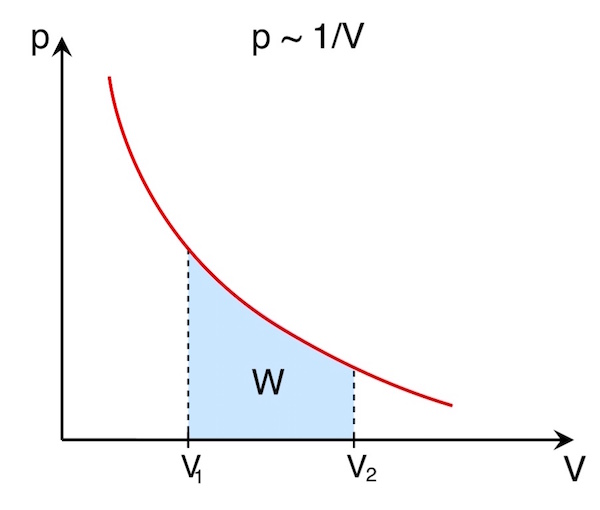
\includegraphics[scale=0.3]{graficos/trab2.jpg}
\end{figure}

\section*{Procesos reversibles}
\addcontentsline{toc}{section}{Procesos reversibles}
\subsection*{Proceso isocórico}
\addcontentsline{toc}{subsection}{Proceso isocórico}
Es aquel donde el volumen es constante, por lo tanto no hay variación de volumen y el trabajo es 0.
\subsection*{Proceso isobárico}
\addcontentsline{toc}{subsection}{Proceso isobárico}
Es aquel donde la presión es constante.Tenemos:
\begin{equation*}
W_{ab} = \int_{V_a}^{V_b} P \cdot dv = P \int_{V_a}^{V_b} dv
\end{equation*}
\begin{equation*}
W_{ab} = P \Delta V = P (V_a - V_b)
\end{equation*}
\subsection*{Proceso isoteŕmico}
\addcontentsline{toc}{subsection}{Proceso isotérmico}
Es aquel donde la temperatura es constante. Aplicando la ecuación de estado (EdE) del gas ideal:
\begin{equation*}
PV = nRT
\end{equation*}
Encontramos distintos casos. 
\subsubsection*{Expansión isotérmica de un gas ideal}
\addcontentsline{toc}{subsubsection}{Expansión isotérmica de un gas ideal}
La presión tiene la forma, despejando de la EdE anterior:
\begin{equation*}
P = \frac{nRT}{V}
\end{equation*}
\begin{equation*}
W= \int_{V_a}^{V_b} P \cdot dv = \int_{V_a}^{V_b} \frac{nRT}{V} dv
\end{equation*}

\vspace{15px}
Como nRT es constante, 
\vspace{1px}
\begin{equation*}
W= nRT\int_{V_a}^{V_b} \frac{dv}{V} = nRT \cdot ln\left(\frac{V_b}{V_a}\right)
\end{equation*}
\subsubsection*{Expansión un gas ideal a temperatura constante}
\addcontentsline{toc}{subsubsection}{Expansión un gas ideal a temperatura constante}
\begin{figure}[H]
\centering
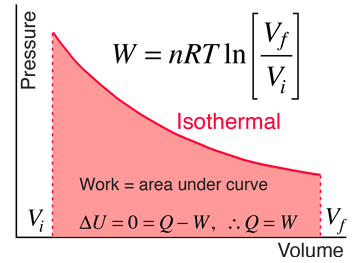
\includegraphics[scale=3]{graficos/t3.png}
\end{figure}
\begin{itemize}
\setlength\itemsep{0.001cm}
\item{Si $V_b > V_a \rightarrow$ Expansión. 
\begin{equation*}
ln\left(\frac{V_b}{V_a}\right) > 0 
\end{equation*}
}
\item{Si $V_b < V_a \rightarrow$ Compresión. 
\begin{equation*}
ln\left(\frac{V_b}{V_a}\right) < 0 
\end{equation*}
}
\end{itemize}

\chapter*{Primer principio de la termodinámica}
\addcontentsline{toc}{chapter}{Primer principio de la termodinámica}
\section*{Experimentos de Joule}
\addcontentsline{toc}{section}{Experimentos de Joule}
Realiza una serie de experimentos para producir un determinado incremento en la temperatura de una masa conocida de agua. 
\begin{figure}[H]
\centering
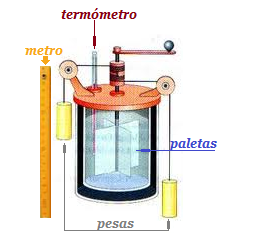
\includegraphics[scale=0.9]{graficos/j1.png}
\end{figure}

Joule demostró que, en condiciones adiabáticas, para pasar de un mismo estado inicial al mismo estado final se requiere la misma cantidad de trabajo, independiente de las particularidades el proceso. 

\section*{Generalización de forma empírica}
\addcontentsline{toc}{section}{Generalización de forma empírica}
El trabajo que se requiere para llevar un sistema rodeado de paredes adiabáticas desde un estado inicial A a otro final depende únicamente de dichos estado.

Cuando i y F son son estados de un sistema conectados mediante un proceso adiabático, existe una función termodinámica, denomináda \textbf{Energía interna (U)}
\begin{equation*}
W_{iF}^{AD} = -\Delta U
\end{equation*}
\todo[inline,backgroundcolor=red!10]{Convencionalmente $\Delta U \rightarrow$ valor negativo del trabajo adiabático ejercido sobre el sistema}
\section*{Calor}
\addcontentsline{toc}{section}{Calor}
\begin{itemize}
\setlength\itemsep{0.001cm}
\item{Energia interna (U): Energia que el sistema puede acumular debido a la propia constitución de la materia. (enlace de las moléculas, interacciones entre ellas, etc}
\item{Calor: En los experimentos no es común hacer evolucionar un sistema solo mediante trabajos cinéticos}
\end{itemize}
Supongamos que se tiene un sistema A, a distinta temperatura del ambiente y se hace evolucionar desde el estado de equilibrio "i" al estado de equilibrio "F". Primero mediante un \textbf{proceso adiabático} desde "i" a "F" y después por cualuier transformación \textbf{NO} adiabática desde "i" hasta "F", es decir, se realiza el mismo cambio de estado. Las conclusiones son:
\begin{itemize}
\setlength\itemsep{0.001cm}
\item{En trans adiabáticas $\rightarrow W = \Delta U$}
\item{En trans NO adiabáticas $\rightarrow W \neq \Delta U$}
\end{itemize} 
Para que el resultado sea compatible con el principio de la conservación de la energía, debe deducirse que hace existido \textbf{Transferencia de energía por medios distintos a la realización de trabajo}. 
A esta 'energía transferida' en forma distinta se denomina 'Calor, flujo de calor' 
\subsection*{Definicion operacional de calor}
\addcontentsline{toc}{subsection}{Definicion operacional de calor}
Energía transferida por medios no mecánicos, durante la evolución de un sistema que puede y cuando el sistema se encuentra a distinta temperatura de su ambiente.

\begin{itemize}
\setlength\itemsep{0.001cm}
\item{Calor: suma de variación de energía interna y del trabajo realizado, es decir, 
\begin{equation*}
Q_{if} = \Delta U + W_{if}
\end{equation*}}
\end{itemize} 
A la ecuación 
\begin{equation*}
\Delta U = Q_{if} - W_{if}
\end{equation*}
Se le conoce como \textbf{El primer principio de la termodinámica}
\subsection*{Capacidad calorífica (C)}
\addcontentsline{toc}{subsection}{Capacidad calorífica (C)}
Si un sistema de masa 'm' absorve un calor 'Q', puede  o no tener lugar un cambio de temperatura, dependiendo del tipo de proceso que acuna. Si en la absorción de calor 'Q' el sistema cambia su temperatura de $T_i$ a $T_f$, entonces estas magnitudes se encuentran a través de la capacidad calorífica media ($\bar{C}$):
\begin{equation*}
\bar{C} = \frac{Q}{\Delta T} [J/K] \rightarrow \displaystyle\lim_{\Delta T \to 0}\frac{Q}{\Delta T} = \frac{d'Q}{dt}
\end{equation*}

\subsection*{Capacidad calorífica a Presión constante}
\addcontentsline{toc}{subsection}{Capacidad calorífica a Presión constante} Capacidad calorífica en un proceso durante el cual, él se somente a una presión hidrostática externa constante
\subsection*{Capacidad calorífica a Volumen constante}
\addcontentsline{toc}{subsection}{Capacidad calorífica a Volumen constante}
 Capacidad calorífica en un proceso donde el sistema a volumen constante, mientras se le suministra calor. 
\subsection*{Calor específico (c)}
\addcontentsline{toc}{subsection}{Calor específico (c)}
Capacidad calorífica por unidad de masa o mol. Es característico de las sustancias que consitutye al sistema y se representa por $c_p$ o $c_V$ (p=cte y v=cte respectivamente). Matemáticamente se define como
\begin{equation*}
c = \frac{C}{n} = \frac{C}{m} [J/knK] [J/KgK]
\end{equation*}
LA cantidad total de calor $Q$ que fluye en un sistema en cualquier proceso viene dado por:
\begin{equation*}
Q = \int d'Q = \int_{T_1}^{T_2}C\thinspace dT 
\end{equation*}
o bien como
\begin{equation*}
Q =\int_{T_1}^{T_2}nc\thinspace dT = \int_{T_1}^{T_2}mc\thinspace dT
\end{equation*}
Dentro de un intervalo de $T_1$ en el cual \textbf{la capacidad calorífica} puede considerarse \textbf{constante:}  
\begin{equation*}
Q =C \Delta T = nc\Delta T = mc\Delta T
\end{equation*}

\section*{Energia interna de un gas ideal}
\addcontentsline{toc}{section}{Energia interna de un gas ideal}
La energía interna de un gas ideal sólo depende de la temperatura. 

\begin{figure}[H]
\centering
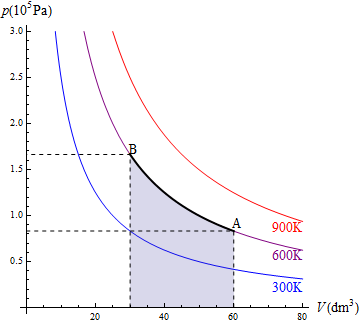
\includegraphics[scale=0.5]{graficos/int.png}
\end{figure}
Un gas ideal sufrirá la misma variación de energía interna $\Delta U_{AB}$, siempre que su temperatura inicial sea $T_A$ y la final sea $T_B$ (Ley de Joule) 

Elegimos una transformación a \textbf{V = cte}
\begin{equation*}
\Delta U_{AB} = Q_{AB} - W_{AB}
\end{equation*}
como $W_{AB}$ = 0
\begin{align*}
\Delta U_{AB} &= Q_{AB} \\
\Delta U_{AB} &= nc_V \Delta T = nc_V(T_B - T_A) 
\end{align*}

\todo[inline,backgroundcolor=green!10]{La ecuación anterior permite calcular $\Delta U$ sufrida por un gas ideal, conocidas $T_i$ y $T_f$ y es válida independientemente de la trayectoria sufrida por el gas.}

\section*{Calor específico de un gas ideal}
\addcontentsline{toc}{section}{Calor específico de un gas ideal}
Procesos que ocurren con frecuencia: Cambios a P=cte y cambios a V=cte. 
\begin{figure}[H]
\centering
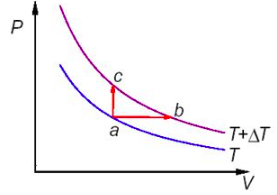
\includegraphics[scale=0.5]{graficos/p1.png}
\end{figure}

\begin{itemize}
\setlength\itemsep{0.001cm}
\item{Para V=Cte (i$\rightarrow c$): 
\begin{equation*}
\Delta U_{ic} = Q_{ic} - W{ic} 
\end{equation*}
Como $W_{ic} = 0$
\begin{equation*}
\Delta U_{ic} = nc_V \Delta T
\end{equation*}}
\item{Para P=Cte (i$\rightarrow b$): 
\begin{align*}
\Delta U_{ib} &= Q_{ib} - W{ib} \\
\Delta U_{ib} &= nc_p \Delta T - P\Delta V
\end{align*}}
\end{itemize}
Luego, por Ley de Joule: 
\begin{equation*}
\Delta U_{ic} = Q_{ic} - W{ic} 
\end{equation*}
Como $W_{ic} = 0$
\begin{equation*}
nc_V\Delta T = nc_p \Delta T - P\Delta T 
\end{equation*}
Vemos que 
\begin{align*}
nc_V\Delta T &= nc_p \Delta T - nR\Delta T \\
c_V &= c_p - R \\
c_p - c_V &= R
\end{align*}

\chapter*{Proceso adiabático reversible}
\addcontentsline{toc}{chapter}{Proceso adiabático reversible}

Supongamos que un gas ideal se somete a una expansión adiabática reversible. 

\textbf{Primer principio:} 
\begin{equation*}
dU = d'Q - d'W
\end{equation*}
Se tiene 
\begin{equation*}
PVT : d'W = P dv 
\end{equation*}

\section*{Proceso adiabático}
\addcontentsline{toc}{section}{Proceso adiabático}
En el proceso adiabático, se tiene $$d'Q = 0, $$ además de $$ dU = -d'W $$ $$ dU = -Pdv  $$
Como la $U$ del gas ideal depende sólo de la temperatura, el cambio en la energía interna es:
\vspace{5px}
\todo[inline,backgroundcolor=red!10]{$$dU = nc_v dT$$}
donde $c_v$ es el calor específico a $V = cte$. 
$$ dT = \dfrac{dU}{nc_v} = -\dfrac{Pdv}{nc_v} $$

\subsection*{Gas ideal}
\addcontentsline{toc}{subsection}{Gas ideal}
El gas ideal se comporta como $PV = nRT,$ las diferenciales totales son 
$$
PdV + VdP = nRdT  
$$
$$
PdV + VdP = nR \left( -\dfrac{PdV}{nc_v} \right)
$$
pero $\left( -\dfrac{PdV}{nc_v} \right) = dT$, por lo tanto 
$$
PdV + VdP = - \dfrac{RPdV}{c_v} 
$$
Sabemos que $c_p - c_v = R$, por lo tanto se define: 
$$
\dfrac{c_p}{c_v}
$$ 
Que es la cantidad , luego 
$$
PdV + VdP = - \frac{(c_p - c_v)PdV}{c_v} /\dfrac{1}{PV}
$$
$$
\dfrac{dV}{V} + \dfrac{dP}{P} = - \frac{(c_p - c_v)dV}{c_v \cdot V} \rightarrow \dfrac{dV}{V} + \dfrac{dP}{P} = (1 - \gamma)\dfrac{dV}{V}
$$
$$
\cancel{\dfrac{dV}{V}} + \dfrac{dP}{P} = \cancel{\dfrac{dV}{V}} -\gamma \dfrac{dV}{V}
$$
$$
d\frac{dP}{P} + \gamma \dfrac{dV}{V} = 0
$$

Al intergrar esta expresión, para un intervalo donde $\gamma$ pueda considerarse constante, resulta: 
$$
ln(P) + \gamma \thinspace ln(V) = cte 
$$
$$
PV \stackrel{\gamma}{=} cte 
$$
La figura muestra el diagrama $PV$ para una expansión adiabática reversible

\begin{figure}[H]
\centering
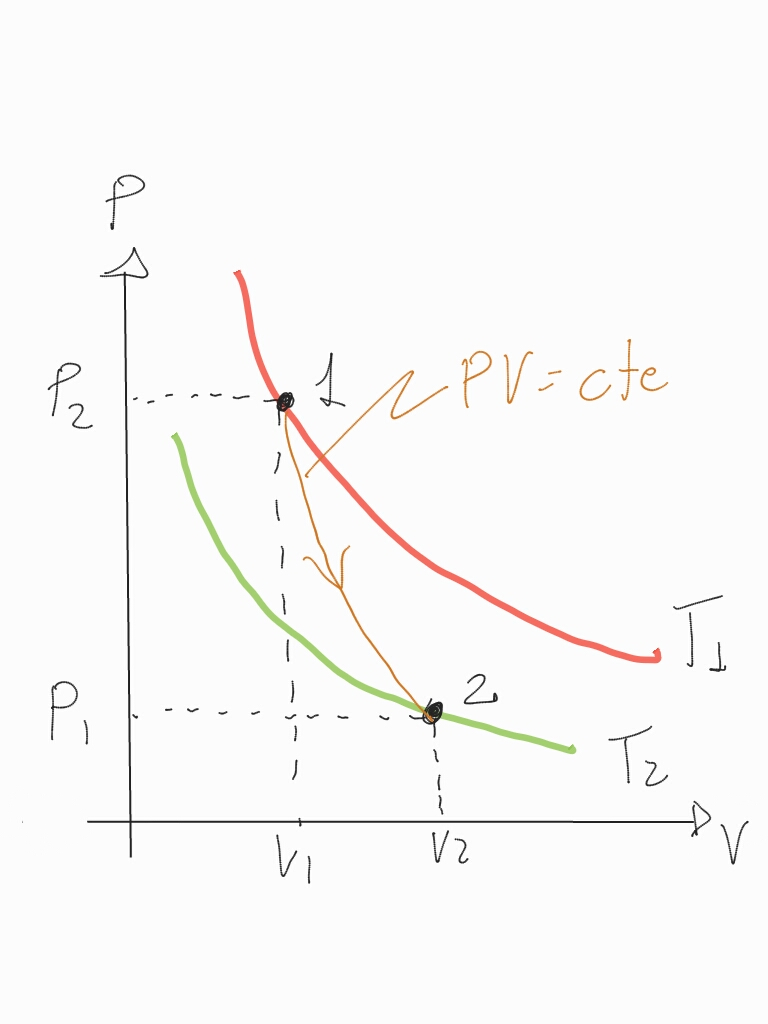
\includegraphics[scale=0.3]{graficos/02_10.jpg}
\end{figure}

\todo[inline,backgroundcolor = green!10]{NOTAS:}
\begin{itemize}
\setlength\itemsep{0.001cm}
\item{Como $\gamma > 1 \rightarrow $La curva $PV$  está más inclinada que para el caso de una expansión isotermica}
\item{El gas se enfría durante una expansión adiabática $(T_2 < T_1)$}
\item{La $T$ aumenta si el gas se comprime de forma adiabática}
\end{itemize}

Al aplicar la ecuación 
$$
PV \stackrel{\gamma}{=} cte 
$$
a los estados iniciales y finales, tenemos que: 
$$
P_1 V_1 \stackrel{\gamma}{} = P_2 V_2 \stackrel{\gamma}{}
$$
que también puede expresarse como:
$$
T_1 V_1 \stackrel{\gamma -1}{} = T_2 V_2 \stackrel{\gamma -1}{}
$$
o también 
$$
T_1 P_1 \stackrel{(1 - \gamma)\gamma}{} = T_2 P_2 \stackrel{(1 - \gamma)\gamma}{}
$$

\subsection*{Trabajo realizado en expansión adiabática reversible con gas ideal}
\addcontentsline{toc}{subsection}{Trabajo realizado en expansión adiabática reversible con gas ideal}
$$
PV ^{\gamma } = cte \rightarrow P = cte \thinspace V^{-\gamma}
$$
Tenemos que 
$$
W = \int_{V_1} ^{V_2} P dV = \int_{V_1} ^{V_2} cte V ^{-\gamma}dV
$$
$$
W = \dfrac{cte}{1 - \gamma} \left[ cte \thinspace V_2 ^{1 - \gamma} - cte \thinspace V_1 ^{1 - \gamma}\right]
$$
$$
cte = P_1 V_1 ^{\gamma} = P_2 V_2 ^{\gamma}
$$
$$
W = \dfrac{1}{1-\gamma} \left[ P_2 V_2 ^{\gamma}V_2^{\gamma - 1} - P_1 V_1 ^{\gamma} V_1^ {\gamma - 1}\right]
$$
\todo[inline,backgroundcolor = green!10]{
$$
W = \dfrac{1}{1- \gamma}\left[P_2 V_2 - P_1 V_1 \right]
$$
}
Lo cual es el área bajo curva roja. 

\section*{Valores para $c_p$ y $c_v$ para gases (T $\approx$ Tambiente}
\addcontentsline{toc}{section}{Valores para $c_p$ y $c_v$ para gases (T $\approx$ Tambiente}
\subsection*{Gases monoatómicos}
\addcontentsline{toc}{subsection}{Gases monoatómicos}
Ejemplo, gases nombres a condiciones normales de Temperatura y presión. 
$$
c_p = \dfrac{5}{2}R
$$
$$
c_v = \dfrac{3}{2}R
$$

\subsection*{Gases diatómicos}
\addcontentsline{toc}{subsection}{Gases diatómicos}
Ejemplo, $H_2, O_2, N_2,$ etc. 
$$
c_p = \dfrac{7}{2}R
$$
$$
c_v = \dfrac{5}{2} R
$$

\subsection*{Gases poliatómicos}
\addcontentsline{toc}{subsection}{Gases poliatómicos}
$$
c_p = 4R
$$
$$
c_v = 3R
$$

\chapter*{Ciclo de Carnot}
\addcontentsline{toc}{chapter}{Ciclo de Carnot}
Corresponde a dos procesos adiabáticos y dos procesos isotéricos. Se supone que un gas ideal contenido en un cilíndro con un élbolo móvil. 

\textbf{Todos los procesos son reversibles}

\section*{Diagrama P-V de un ciclo de Carnot}
\addcontentsline{toc}{section}{Diagrama P-V de un ciclo de Carnot}

\begin{figure}[H]
\centering
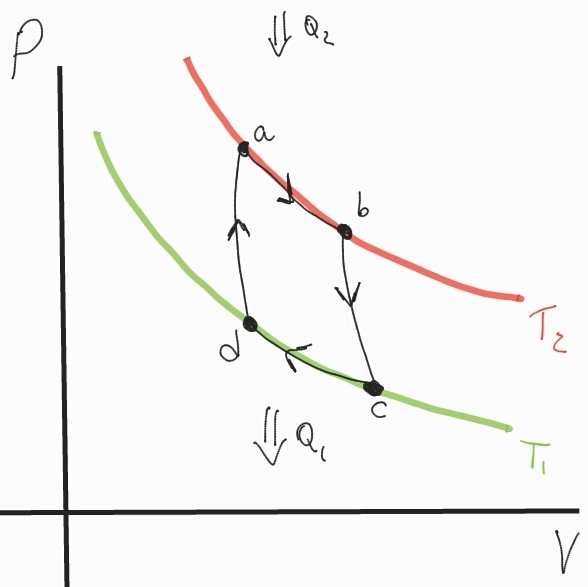
\includegraphics[scale=0.35]{graficos/1_04_10.jpg}
\end{figure}

\subsection*{Proceso a-b $\rightarrow$ isotérmico  }
\addcontentsline{toc}{subsection}{Proceso a-b $\rightarrow$ isotérmico}
Expresión isotérmica a temperatura $T_2$, en la cual el gas se pone en contacto con un depósito de calor que está a temperatura entre proceso, el gas absorbe el calor $Q_2$ del depósito y realiza un trabajo $$W_{ab} = nRT_2 \thinspace ln\left(\dfrac{V_b}{V_a}\right)$$

\subsection*{Proceso b-c $\rightarrow$ Adiabático }
\addcontentsline{toc}{subsection}{Proceso b-c $\rightarrow$ Adiabático}
El gas se expande de manera adiabática ($Q = 0$). La temperatura desciende hasta un valor inferior $T_1$. El gas realiza un trabajo $W_{bc}$ al levantar el émbolo

$$ W_{bc} = \dfrac{1}{1-y} \left[ P_c V_c - P_b V_b \right] $$

\subsection*{Proceso c-d $\rightarrow$ Isotérmico }
\addcontentsline{toc}{subsection}{Proceso c-d $\rightarrow$ Isotérmico}
El gas se pone en contacto con un depósito de calor a temperatura $T_1$ y se comprime isotérmicamente a la temperatura $T_1$. Durante este tiempo, el gas expulsa (libera) el calor $Q_1$ hacia el depósito y el $W$ realizado sobre el gas es 

$$ W_{cd} = nRT_1  \thinspace ln\left(\dfrac{V_d}{V_c}\right) $$

\subsection*{Proceso d-a $\rightarrow$ adiabático }
\addcontentsline{toc}{subsection}{Proceso d-a $\rightarrow$ adiabático}
Se comprime el gas de forma adiabática ($Q=0$). La temperatura del gas aumenta a $T_2$ y el $W$ realizado sobre el gas es 

$$ W_{da} = \dfrac{1}{1-y} \left[ P_a V_a - P_d V_d \right] $$













\end{document}
Esta ultimo ecuación es para gases ideales ($\approx$ gases reales)